\documentclass{jsarticle}

\title{75th2600内装引き継ぎ}
\author{75th621 千葉森生}

\usepackage[dvipdfmx]{graphicx}
\usepackage{subfigure}


\begin{document}

\maketitle

\section{まえがき}

入試を間近に控えておきながら今更2年生の引き継ぎを書いているのは、3年のはいいから2年の時の引き継ぎをかけと急かされている私、内設チのライド担当の千葉でございます。

軽くプロフィール(肩書き自慢)を書くと、以下のようになります。
\begin{itemize}
    \item 75th2600, 3600内装設計チーフ
    \item 75th2600原案班
    \item エンジニアチームCTO
    \item 帰宅部 etc...
\end{itemize}

で、どんな内装を作ったかと言いますと、

\begin{figure}
    \centering
    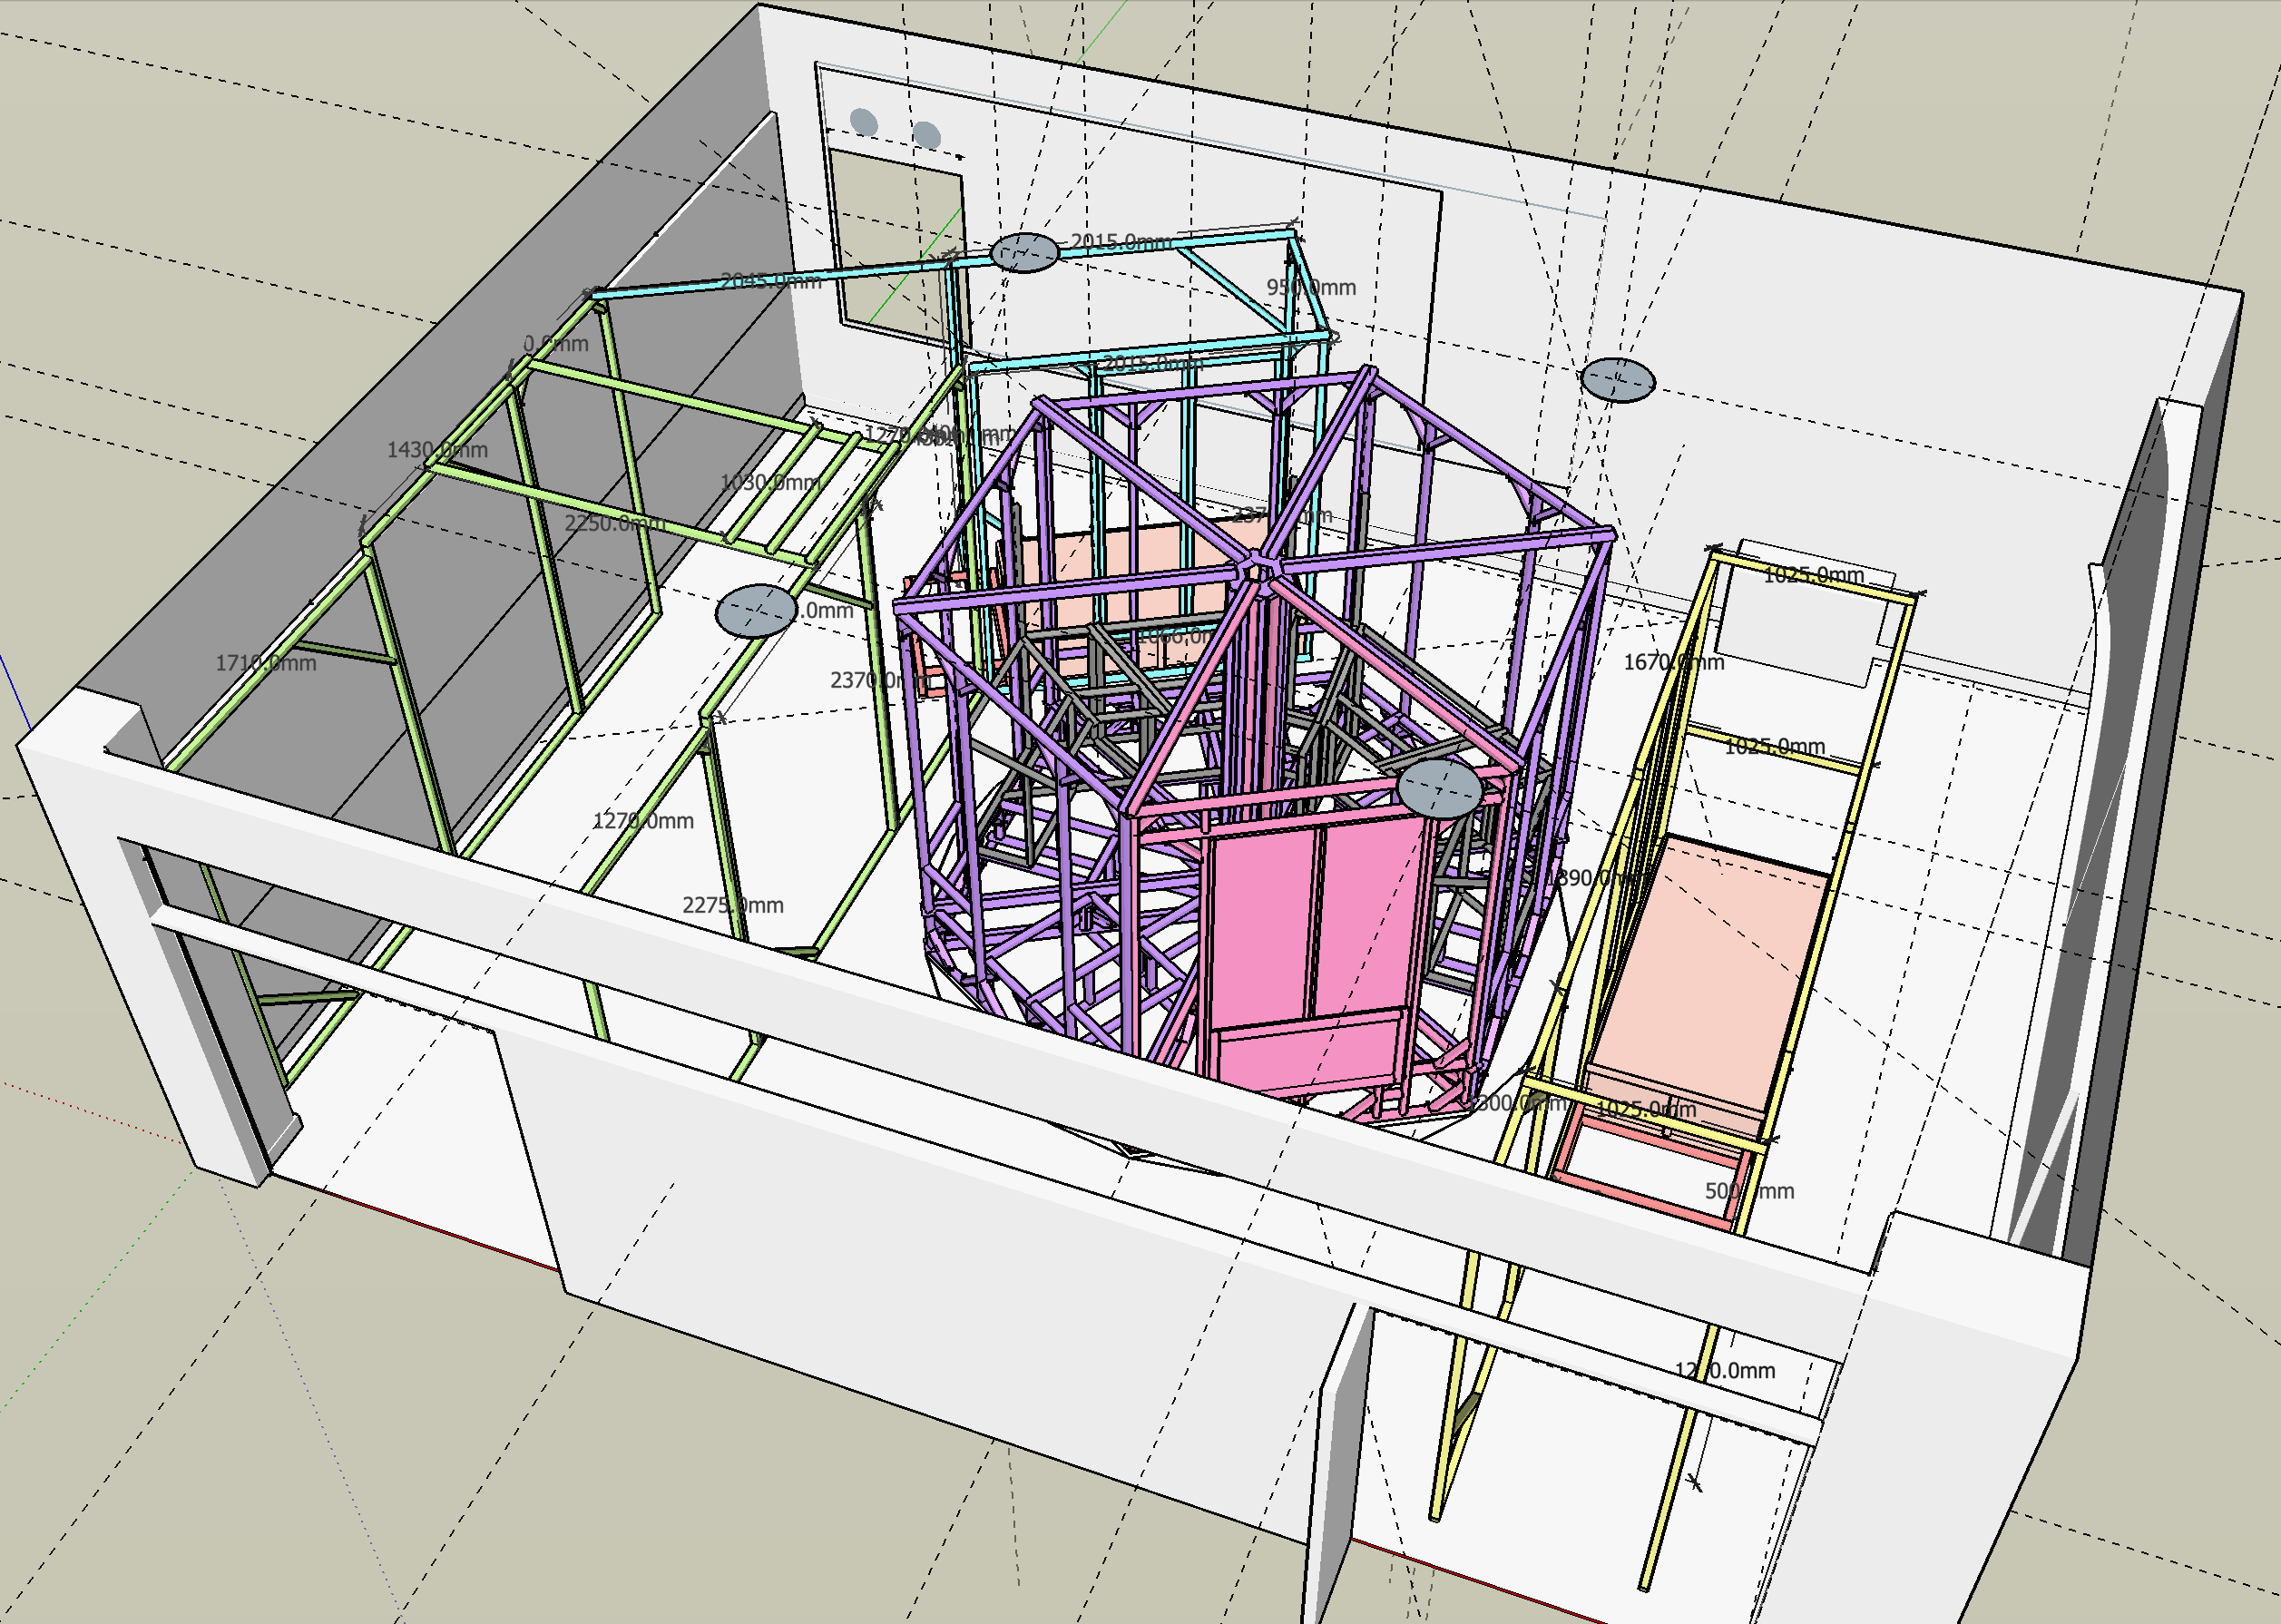
\includegraphics[width=0.8\linewidth]{images/plan_overview/1.png}
    \caption{設計概観}
    \label{fig:設計概観}
\end{figure}

こんなのです。真ん中の正六角形に人を2,3人乗せて回しました。そのため、その辺りの補強が割とエグいです。
今後ライドをやるクラスの参考になれば幸いです。
なお、設計チーフの身ながら内チの仕事に近いところまで手を伸ばしていたので、割と手広い引き継ぎになってます。

疑問点等あればこちらのメールアドレスまでお気軽に:  chibam496@gmail.com

\tableofcontents
\clearpage

\section{概要}
\subsection{成果物}

まずは作ったものの紹介から。

\begin{figure}[h]
    \centering
    \subfigure[完成形]{
        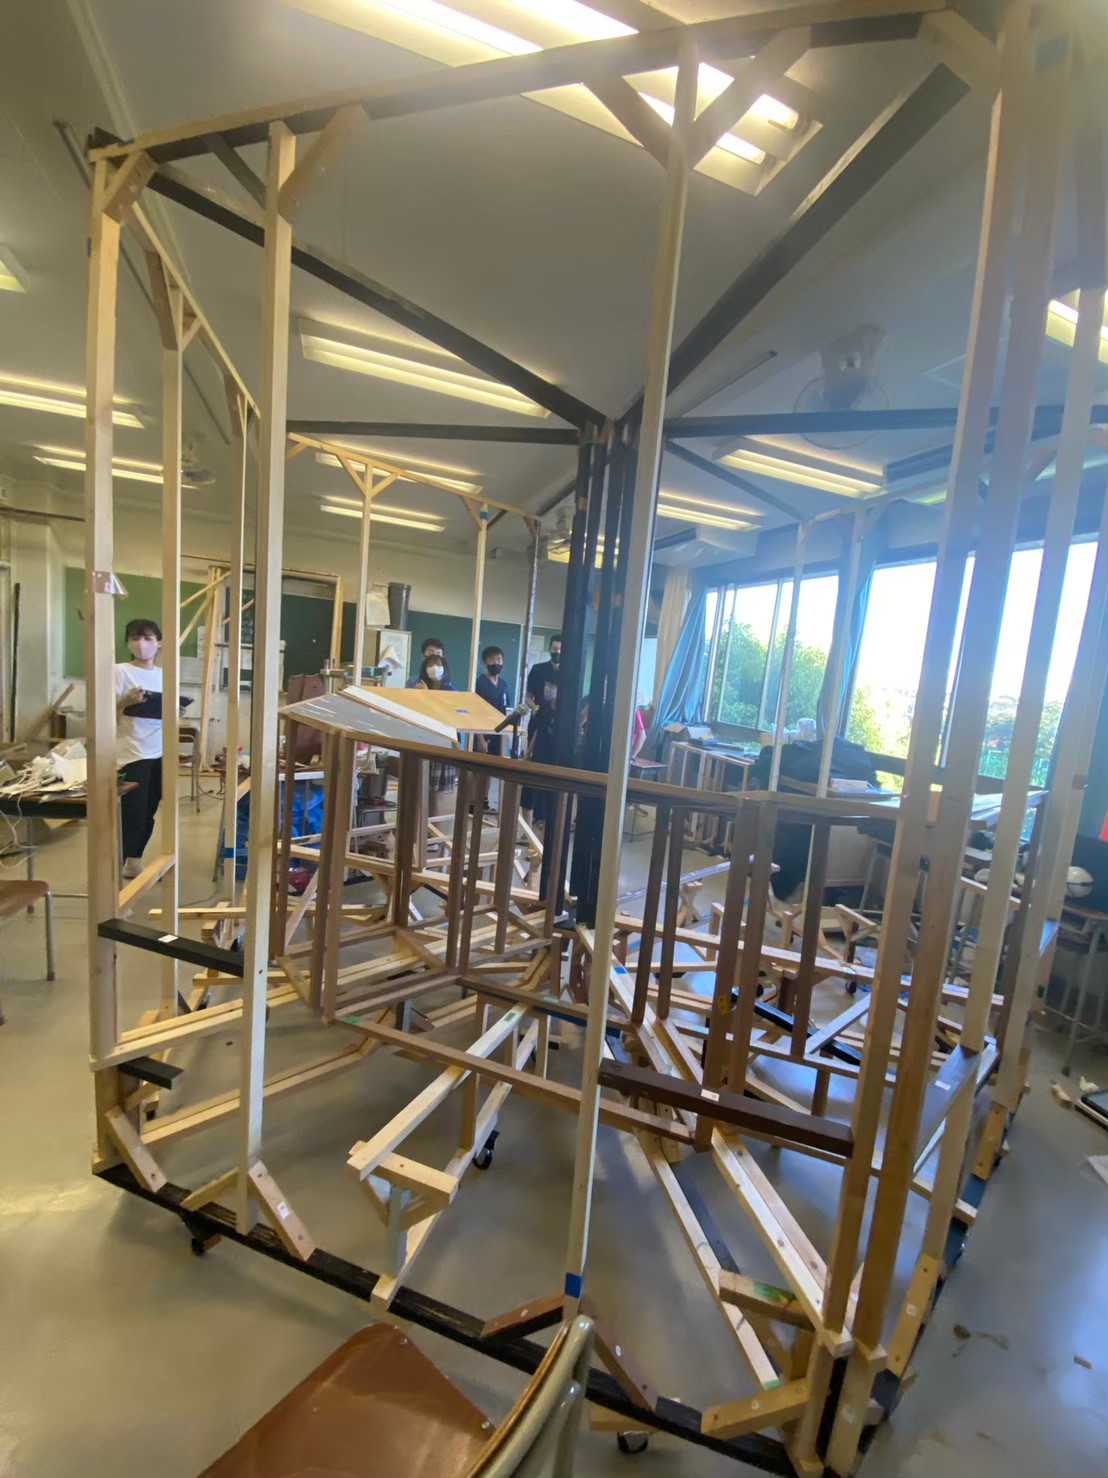
\includegraphics[width=0.45\textwidth]{images/plan_overview/2.jpg}
        \label{fig:完成形}
    }
    \subfigure[完成直前]{
        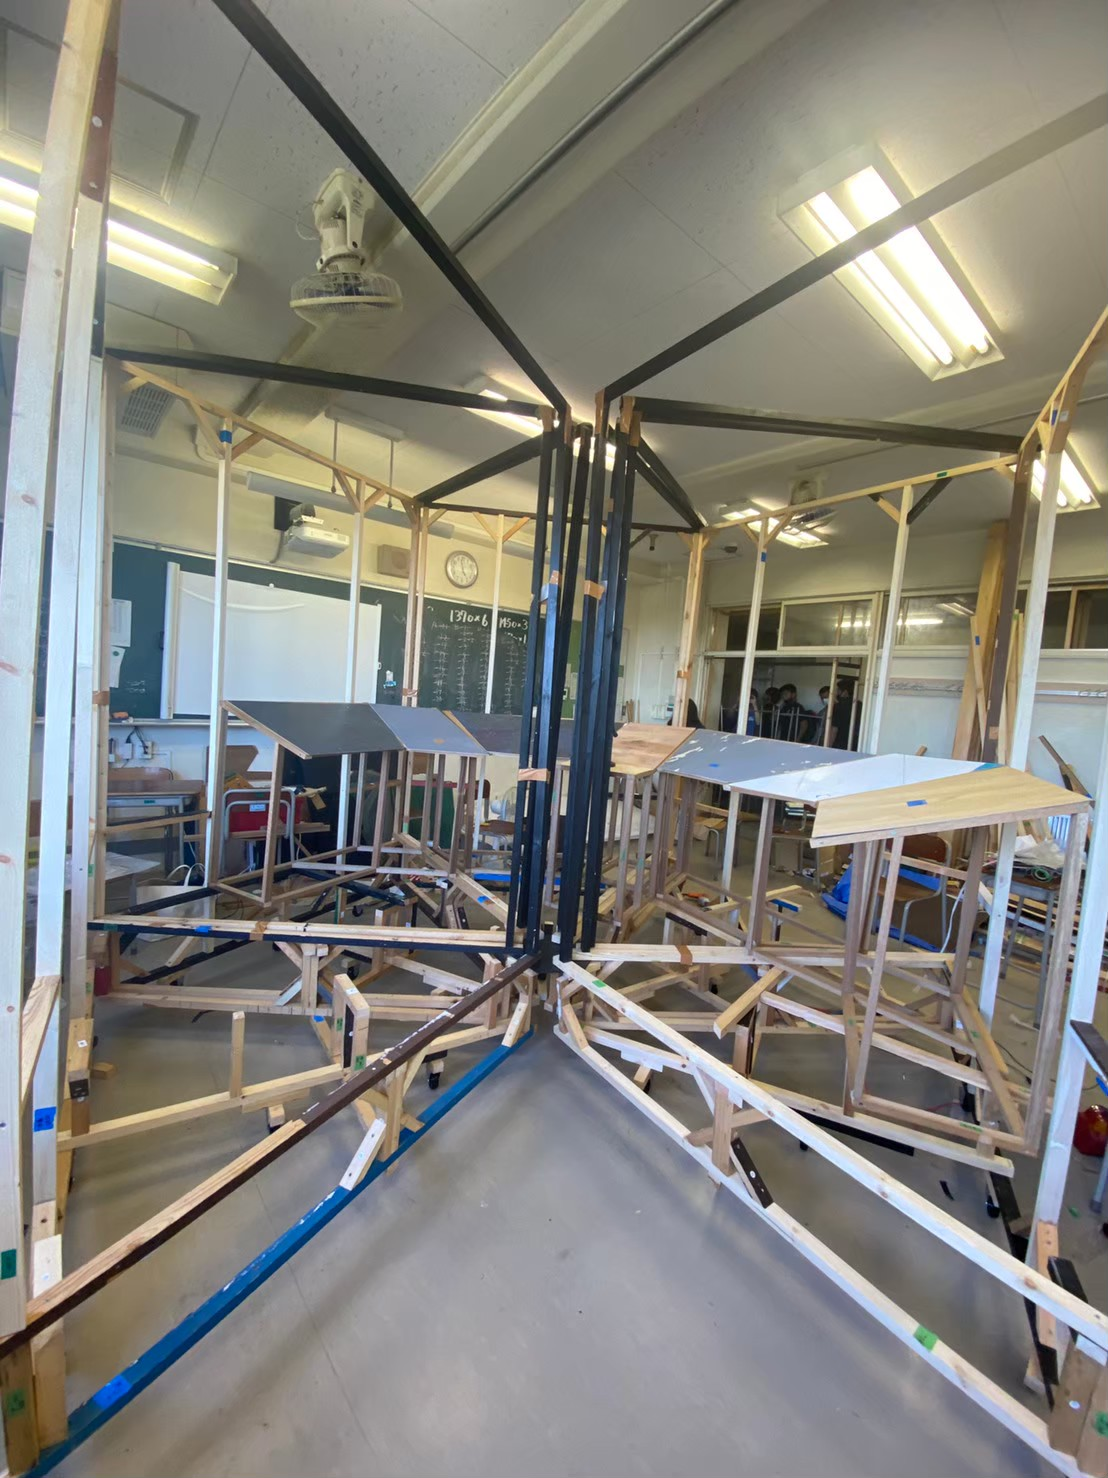
\includegraphics[width=0.45\textwidth]{images/plan_overview/3.jpg}
        \label{fig:完成直前}
    }
    \caption[]{骨組み}
    \label{figs:骨組み}
\end{figure}

正三角形のパーツを6個作り、ネジで繋ぎ合わせて作りました。後述しますが、分割して組み立てる方法は「教室復元」を意識したものなので、似たようなのを作る場合はまとめて作ってしまってもいいと思います。
特徴としては、稼働部が巨大であること、それに応じて補強も複雑であることです。


\begin{figure}[h]
    \centering
    \begin{minipage}{0.45\textwidth}
        \centering
        \subfigure[宇宙船の内装]{
            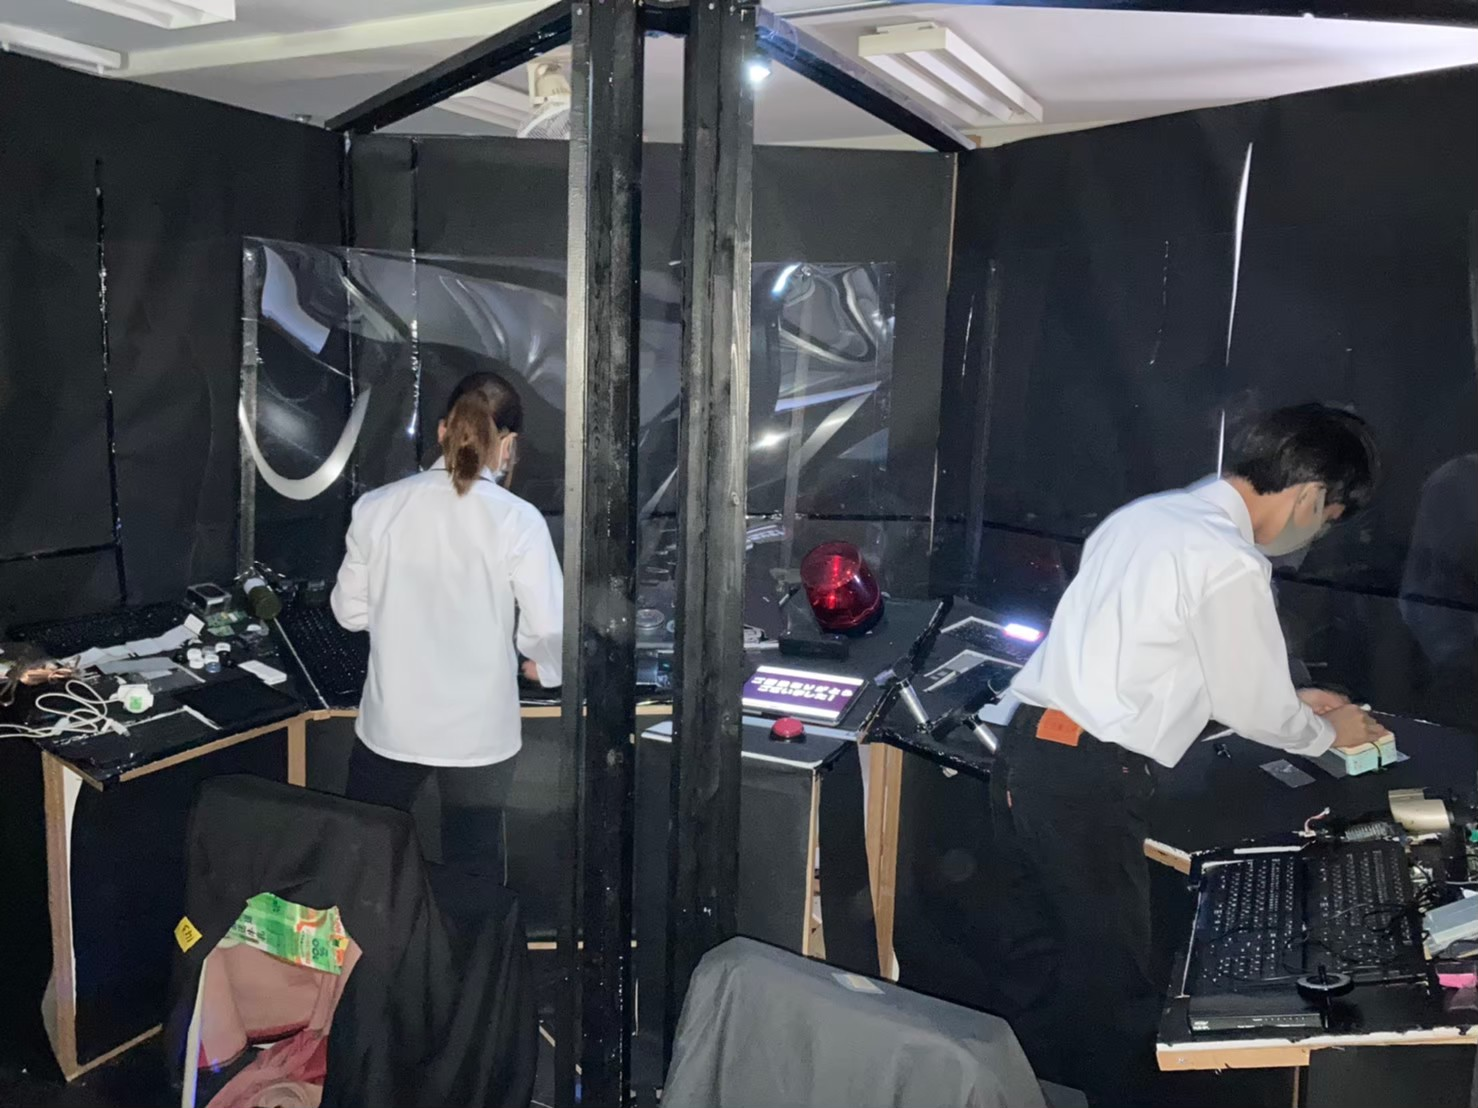
\includegraphics[width=\textwidth]{images/plan_overview/4.jpg}
            \label{fig:内装}
        }
        \subfigure[降りた後の通路から出口方面]{
            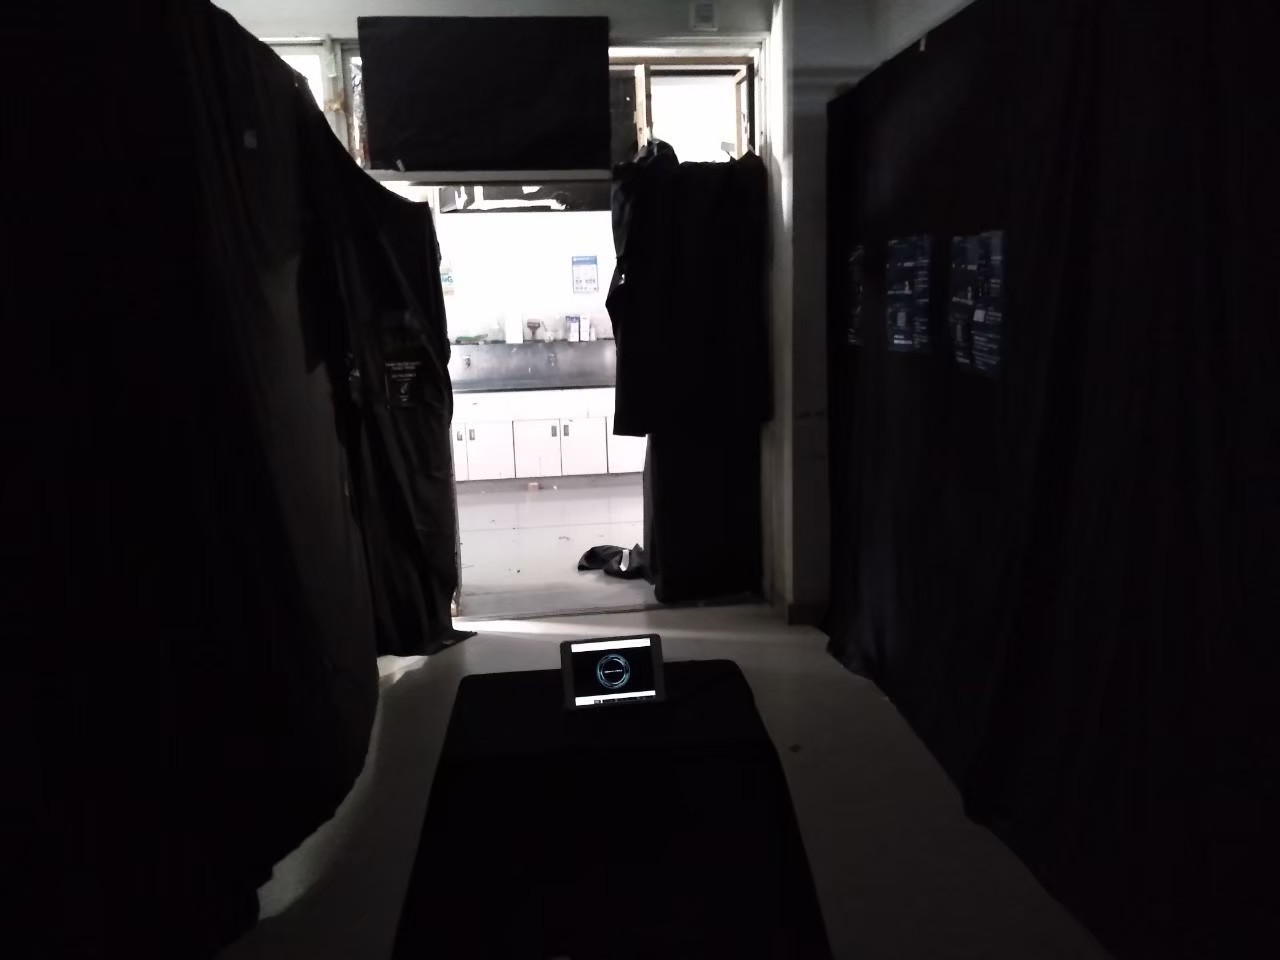
\includegraphics[width=\textwidth]{images/plan_overview/5.jpg}
            \label{fig:出口}
        }
    \end{minipage}\hfill
    \begin{minipage}{0.45\textwidth}
        \centering
        \subfigure[ライドを動かす様子]{
            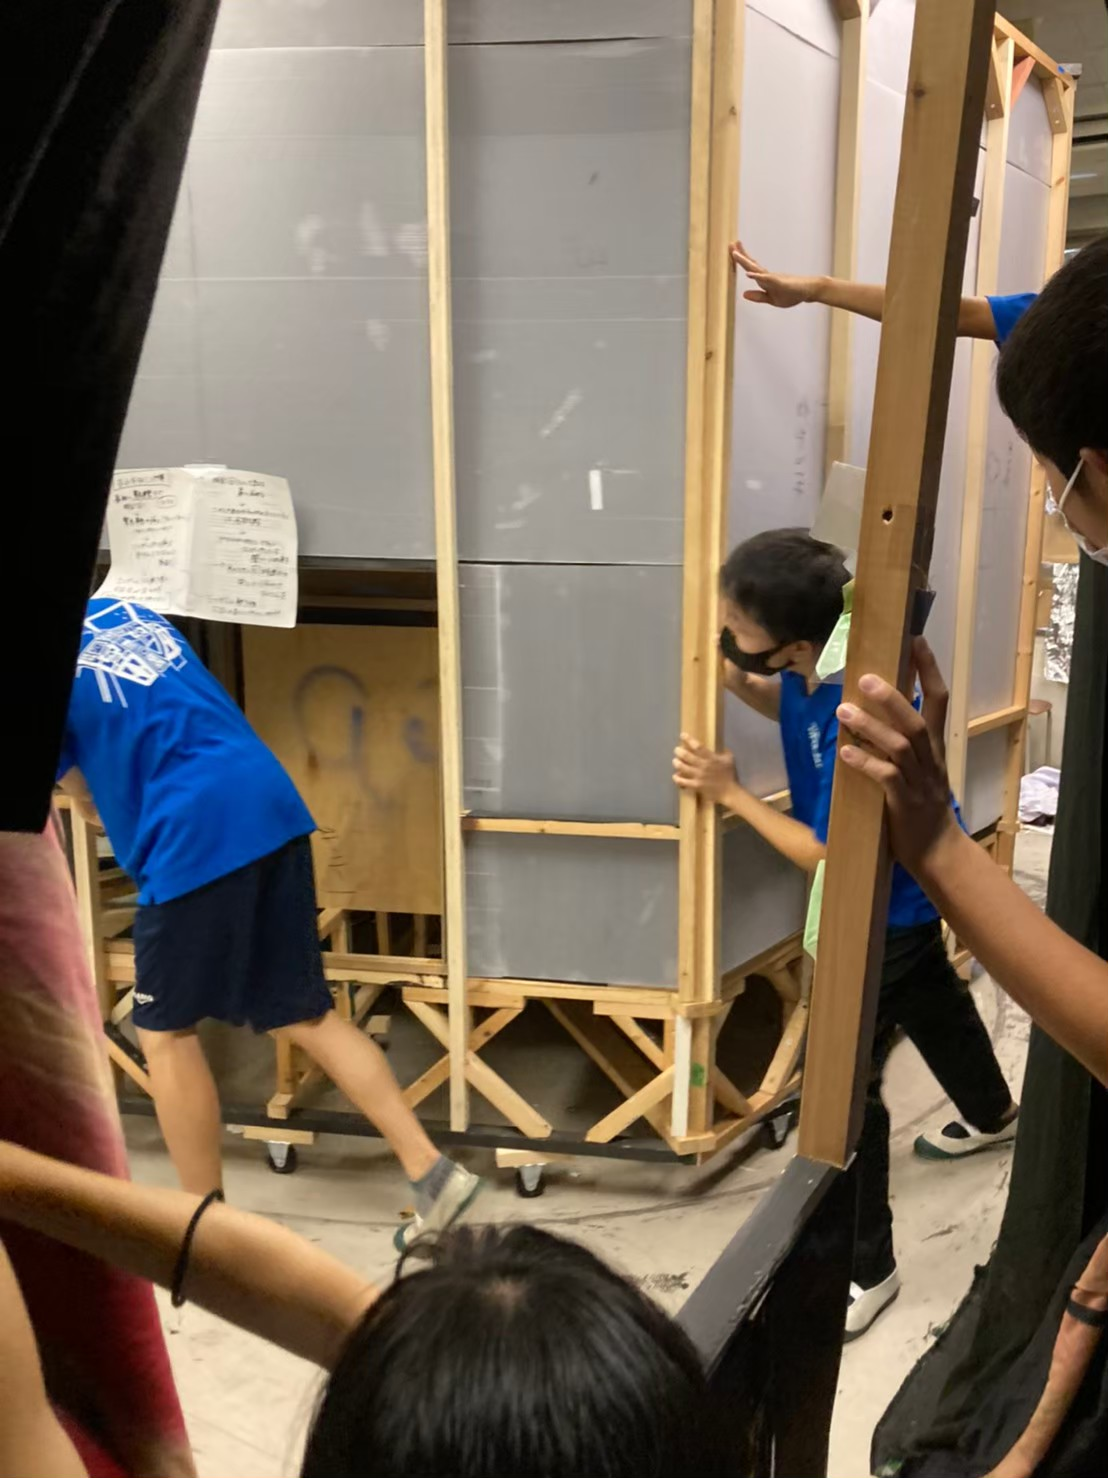
\includegraphics[width=\textwidth]{images/plan_overview/6.jpg}
            \label{fig:人力}
        }
    \end{minipage}
    \caption[]{装飾後}
    \label{figs:装飾後}
\end{figure}

基本的に二人乗りですが、動き回ることを想定しているので実際は5人ぐらい入っても問題ない大きさ。もっとも、ライドを回すのは人力なので、あまり重いと回りませんが。

\clearpage

\subsection{動線}

\begin{figure}[h]
    \centering
    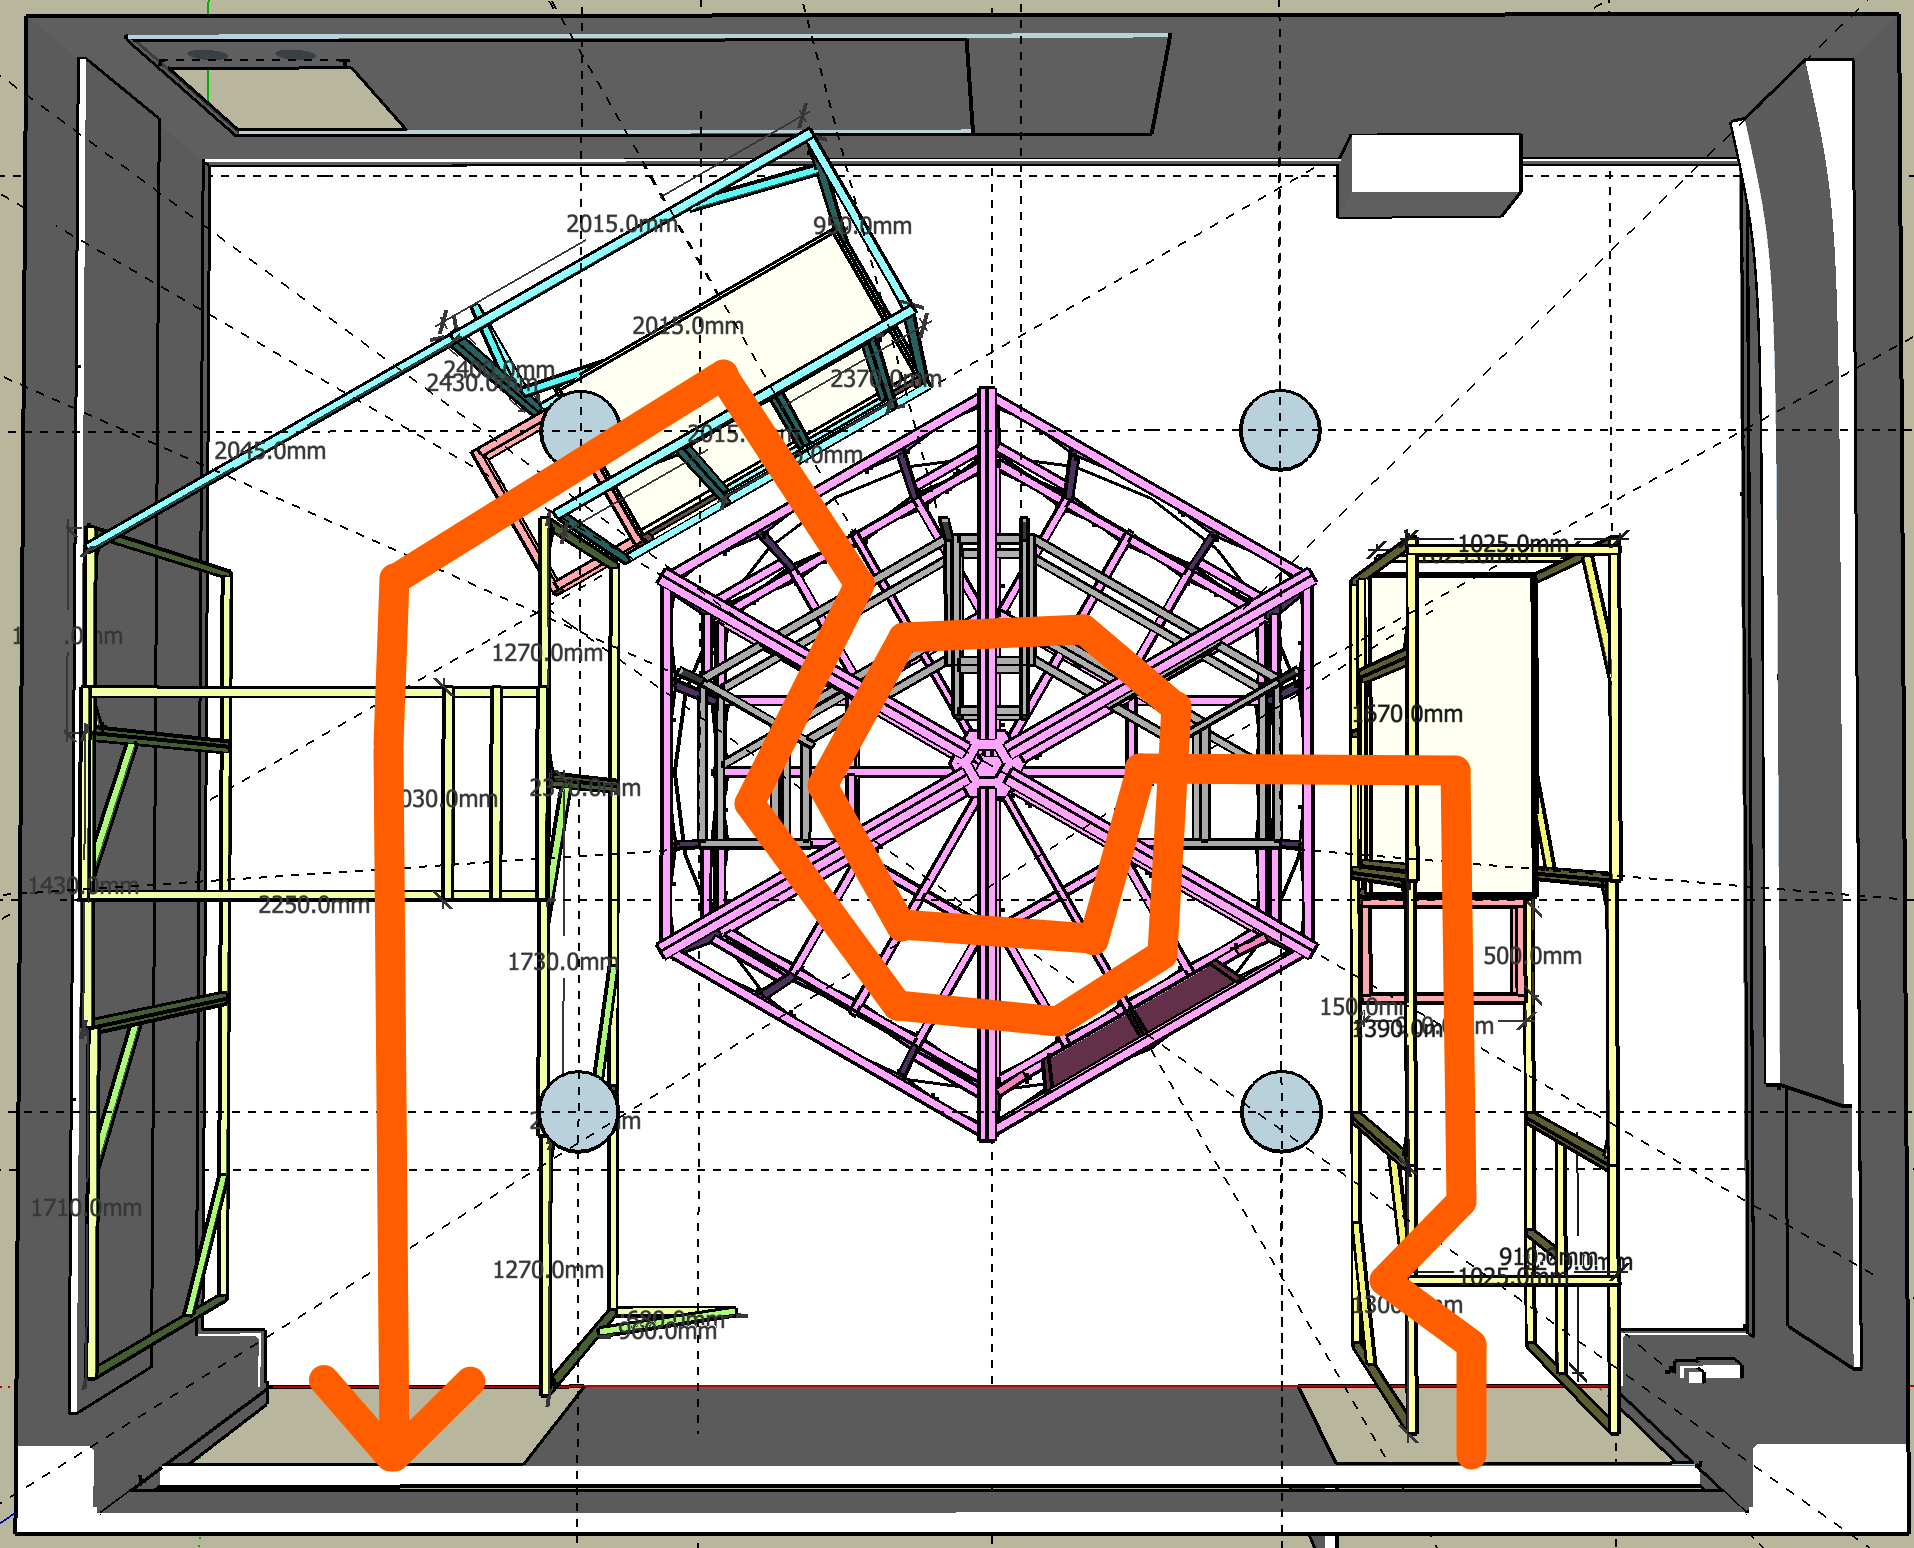
\includegraphics[width=0.6\linewidth]{images/lane.png}
    \caption{動線}
    \label{fig:動線}
\end{figure}

\begin{enumerate}
    \item 教室前方のドアが入り口、入って左側に受付
    \item そのまま進み、渡し板を渡って宇宙船に乗り込む
    \item ミニゲームを解く間に、ストーリーに合わせて宇宙船が回転
    \item 宇宙船から降りた後、出口側の通路でミニゲームの結果に応じた映像を流す
    \item 教室後方から出て終了
\end{enumerate}

\section{案の確定に至るまで}

\subsection{第1回プレゼン大会@Jan 13 (原案班)}

我々のクラスでは、近くの席の人と数人ずつグループになって案を考え、2回のプレゼンを経て最終案を決定しました。
初期の案では、4組が同時に参加できる方式を考えていました。4つの少しずつ異なる部屋を用意して相互に連結し、レールの上を回す、というアイデアです。
ミニゲームについては具体的に決めず、クラスから公募する方針でした。
この段階で、プレゼンに向けてBlenderを用いて3Dモデルを作成しました。
具体的なサイズなどが感覚的にわかるため、これはかなり良かったです。sketchupでも構わないので作るといいと思います。

\begin{figure}[h]
    \centering
    \subfigure[企画書]{
        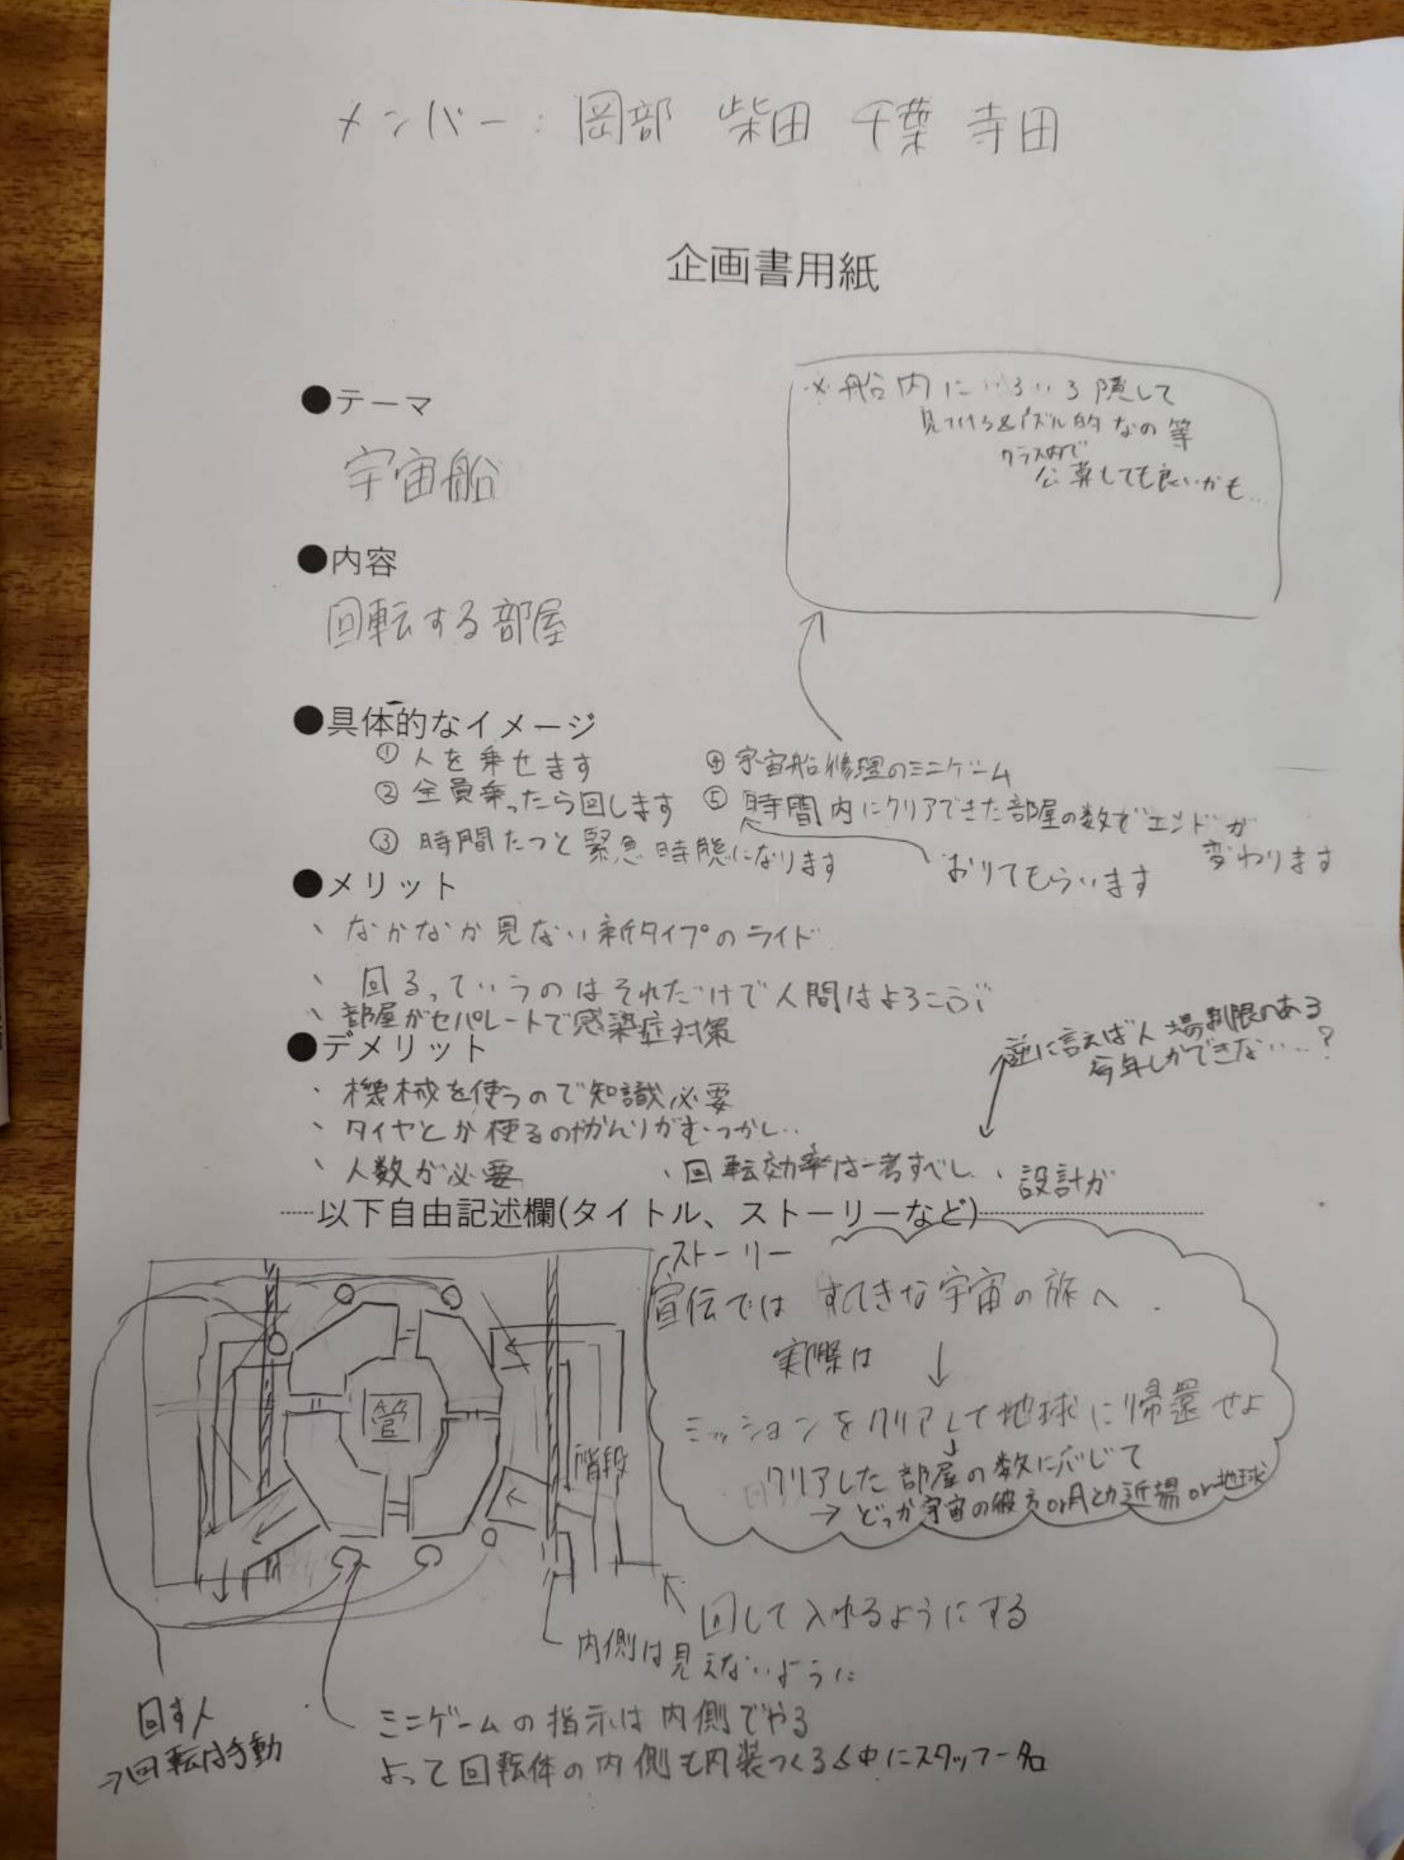
\includegraphics[width=0.45\linewidth]{images/original_plan.png}
        \label{fig:企画書}
    }
    \subfigure[3Dモデル]{
        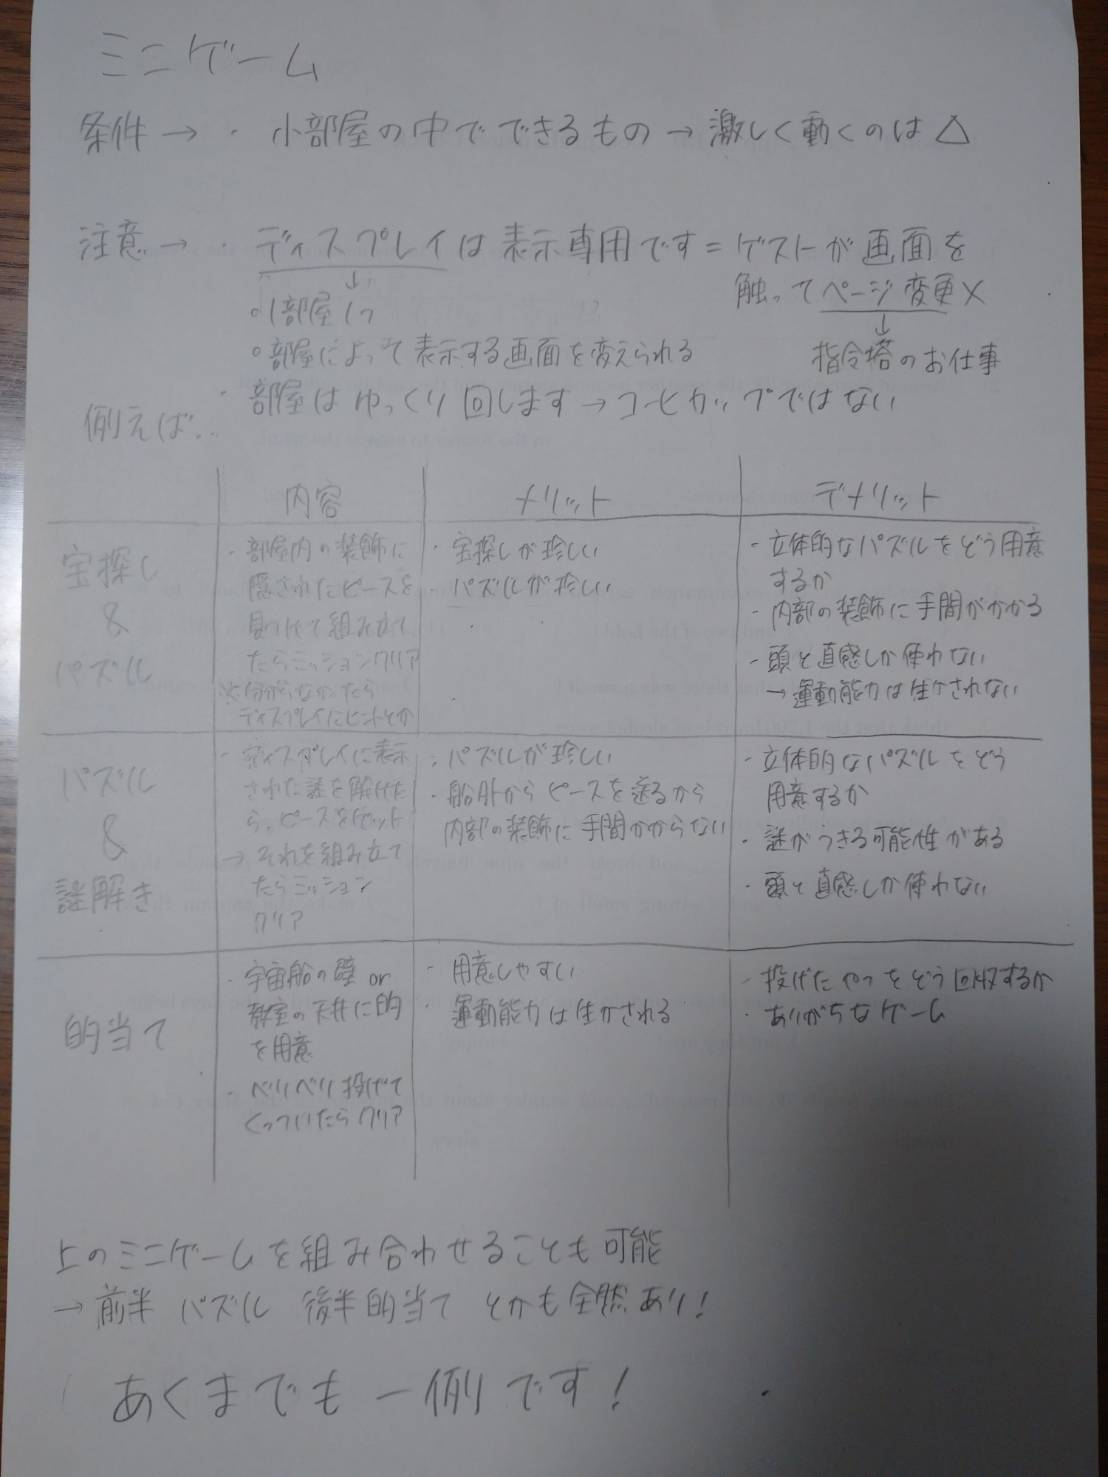
\includegraphics[width=0.45\linewidth]{images/minigame.jpg}
        \label{fig:3Dモデル}
    }
    \caption{原案1}
    \label{figs:原案1}
\end{figure}


\subsection{第2回プレゼン大会@Feb 10 (原案班)}

\begin{figure}[h]
    \centering
    \subfigure[ミニゲームについて]{
        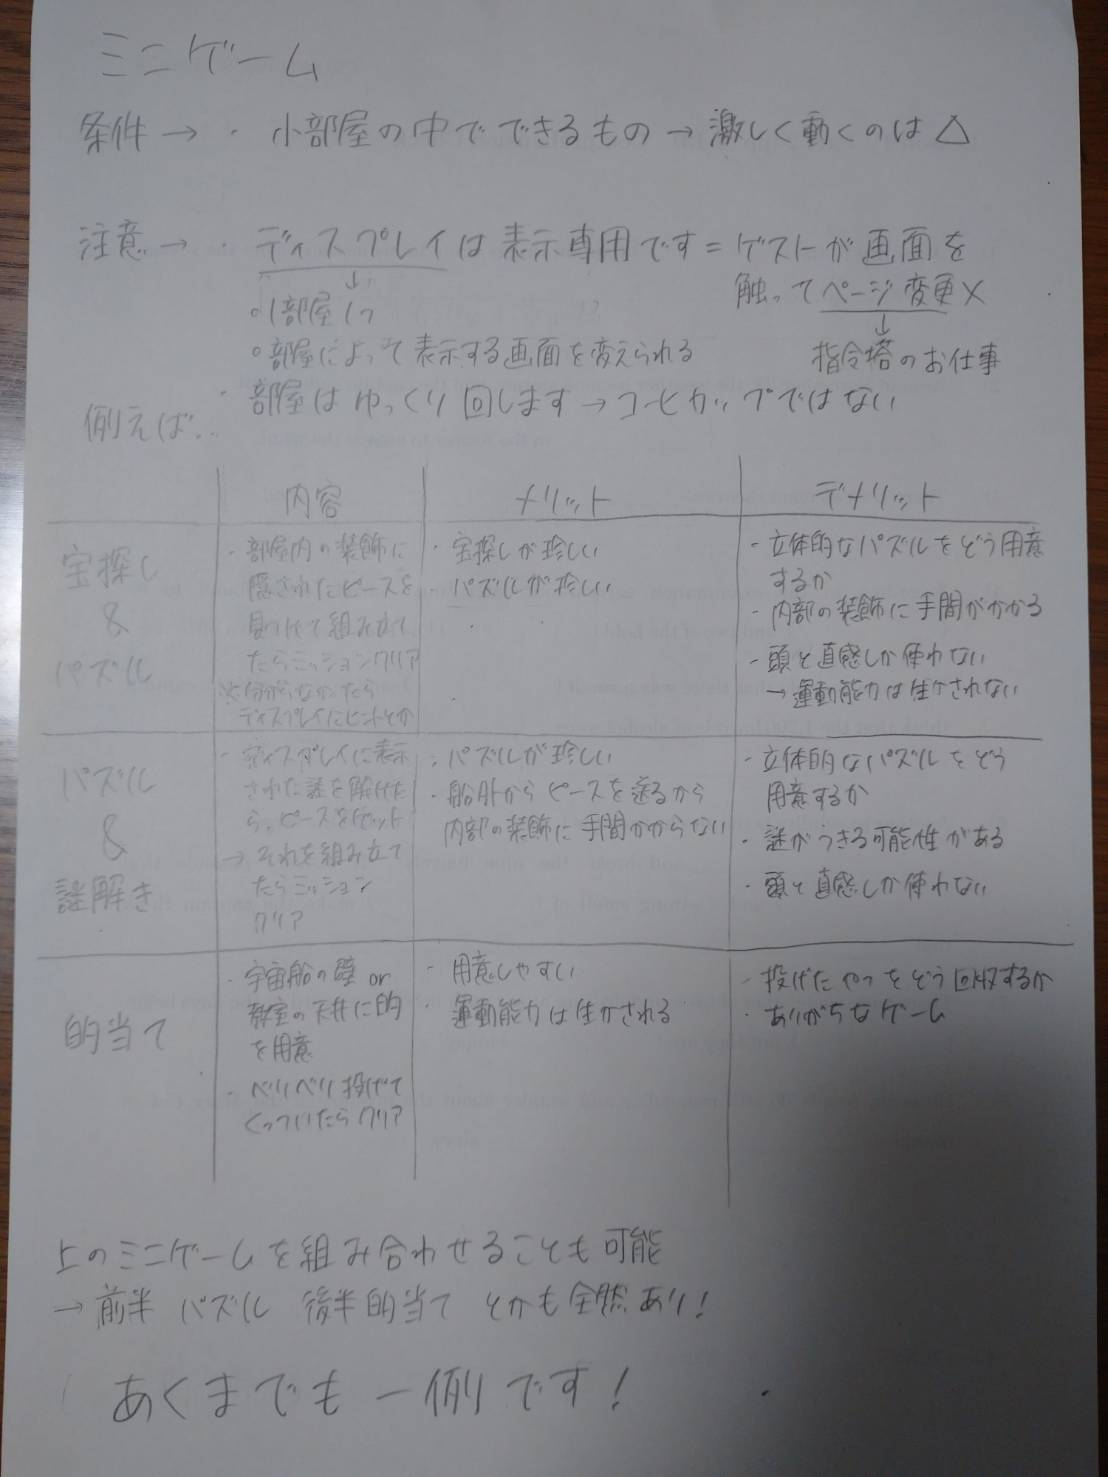
\includegraphics[width=0.45\linewidth]{images/minigame.jpg}
        \label{fig:ミニゲーム}
    }
    \subfigure[質問]{
        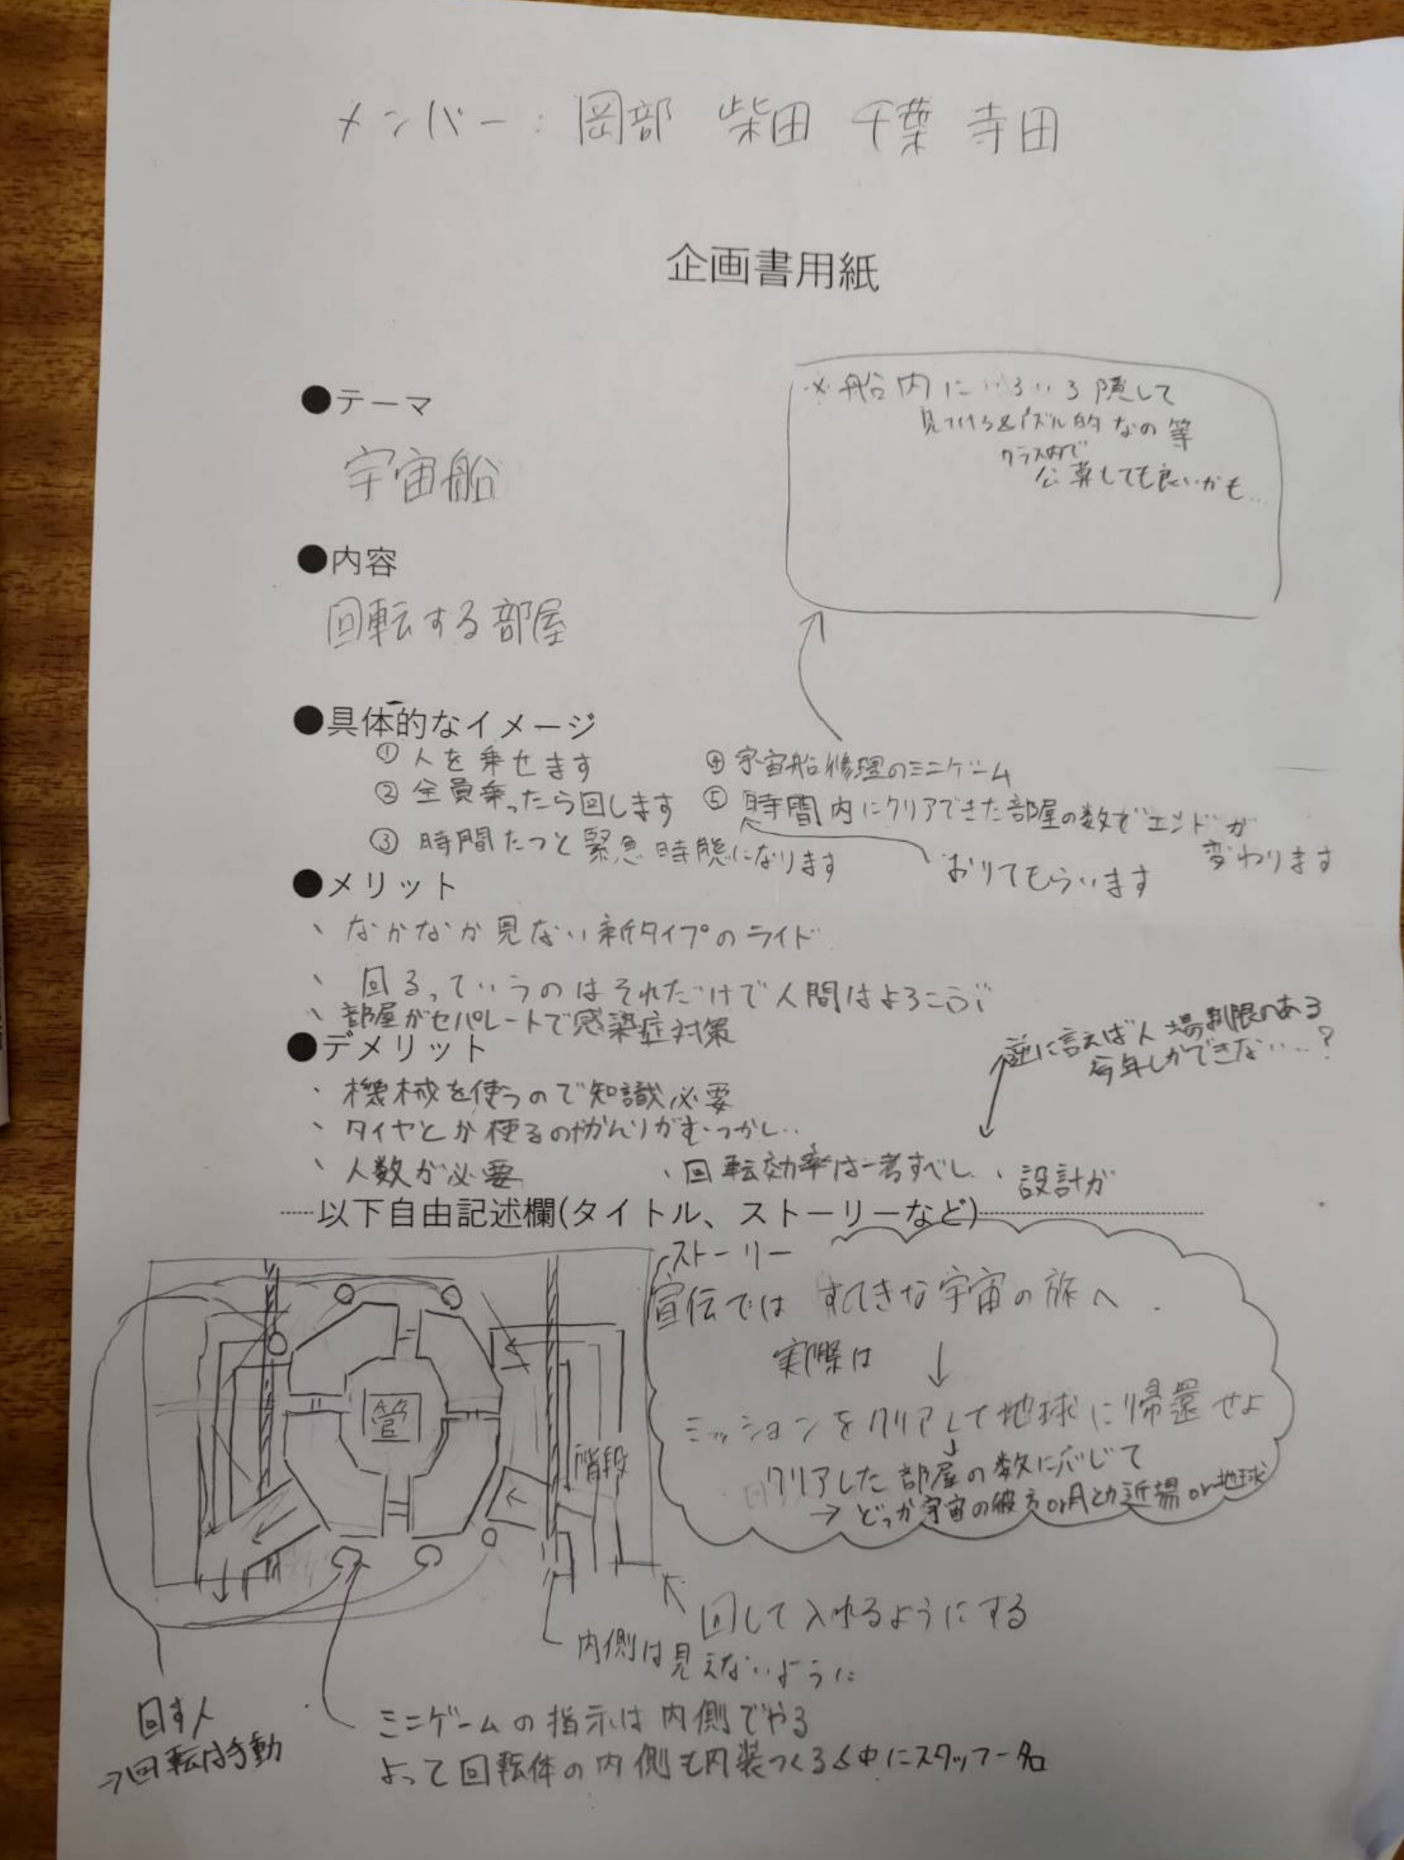
\includegraphics[width=0.45\linewidth]{images/original_plan.png}
        \label{fig:質問}
    }
    \caption{原案2}
    \label{figs:原案2}
\end{figure}

\clearpage

\subsection{展示決定@Mar 3}
\subsection{ストーリー草案@Mar 19}

\clearpage

この案で決定はしたものの、以下のように解決し難い問題が多数浮上したので、一つの箱を4個に分割する案に移行しました。

\begin{itemize}
    \item 十分な耐久性、安定性のあるレールが低コストでは作れない
    \item 連結部の耐久性が確保できない
    \item スペースに無駄が多い (中央の空間を管制塔みたいに使う案もあった)
\end{itemize}

\subsection{ミニゲーム公募@Mar 22}

\section{骨組みについて}

\url{http://yensosha.blog53.fc2.com/blog-entry-592.html}
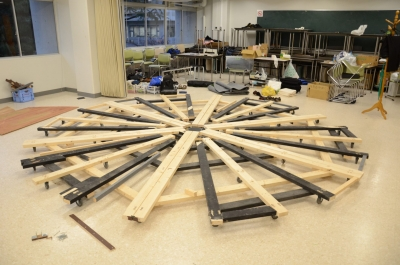
\includegraphics[]{images/base_bone_1.jpg}

\end{document}